\documentclass[../../ASSD_TP1_G7.tex]{subfiles}
\begin{document}

\chapter*{Introducci\'on}
En el presente informe se analizan las consecuencias de tres maneras de muestrear una se\~nal :
\begin{itemize}  
\item  Con sample and hold
\item  Con llave analógica
\item Con llave analógica y sample and hold 
\end{itemize}
Para realizar el análisis se armo un circuito con el siguiente diagrama de bloques y también se dise\~no un programa en GNU radio para simularlo y poder contrastar resultados:

\begin{figure}[H]
  \centering
   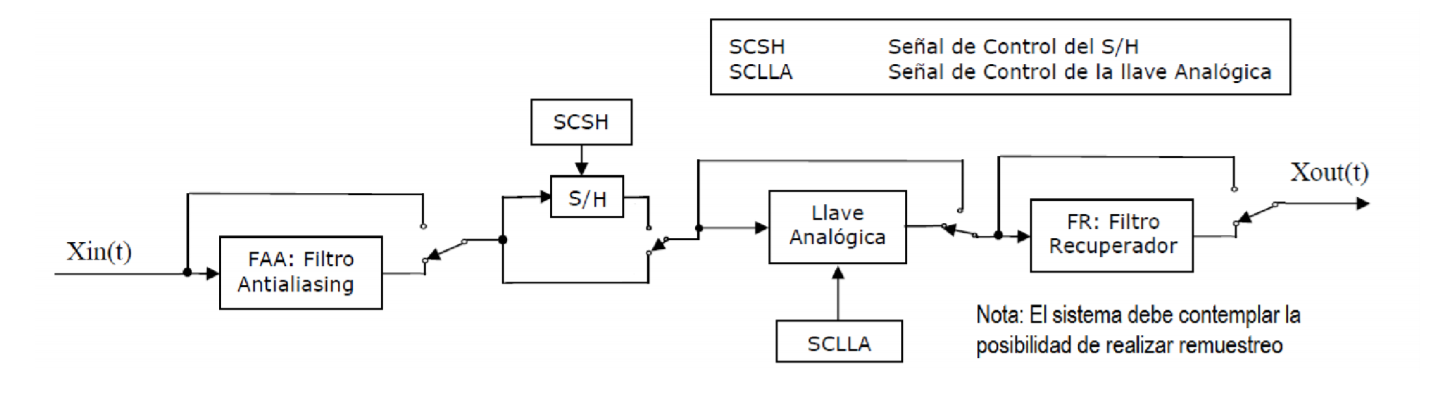
\includegraphics[width=0.9\textwidth]{figures/circuitroBloques.PNG}
  \caption{Diagrama en bloque}
  \label{fig:blocDiagram}
\end{figure}

\par Ademas de analizar los efectos de distintos tipos de muestro, se analizaron las implicancias de en una misma placa combinar circuitos analógicos y digitales.

\end{document}
